\documentclass[../document.tex]{subfiles}

\begin{document}

\section{Sprint 1}

\subsection{Introduction}
The following chapter includes all the documentation regarding the first sprint. The sprint will take place from September 22 and conclude October 3. This gives the team two working weeks to create the initial implementation and prototype.

\subsection{Sprint Planning}
We plan on spending 200 hours for this sprint on implementation and 150 hours on documentation, which includes pre-study if any, meetings and actual sprint documentation. With this, we have a total of 350 working hours over two working weeks and 7 members. Therefore the expected workload for each member is 25 hours per week. Our plan is to create a working prototype within the first sprint and then as agile development continues the cycle improve on it. The team will split into three units, one unit will work on the client, another will work on the database and the last will work on the visualization. We plan on utilizing the pair programming technique and to split 6 people into three teams of two. The last person will be in charge of overviewing documentation and joining any of the teams if they need help.

\subsection{Sprint Goal}
The goal of the first sprint is to create a client, database and a simple visualization method that can be used to test our implementation. Therefore we have three goals:
\begin{enumerate}
\item
Create a client that will be able to fetch data from the central hub and store this data into the database.
\item
Create a database that will be able to store values that the client passes to it.
\item
Create a Table View, which will enable us to fetch data from the database and visualize it on the computer, in the form of a table.
\end{enumerate}
These three goals also coincide with our functionalities and it is vital that these are implemented first. The entire process is described in the architecture, while the table view is described in the requirements part.

\subsection{Sprint Backlog}
Below is the sprint backlog in the form of a table, listing all of the tasks we plan on working on in this sprint. We also include the estimated working hours for each task as well as the actual amount of work spent on each task, as we complete the tasks in the sprint. The tasks also include priority, which will help the group direct their focus on the most important sub-tasks first.


\begin{table}[H]
\caption{Scenario P1}
\begin{tabularx}{\textwidth}{|l|X|l|l|l|}
\hline
Item
&Task
&Priority
&Estimated hours
&Actual hours
\\ \hline1.1
&Design client-central hub interface
&H
&4
&4
\\ \hline1.2
&Implement client-central hub interface
&H
&8
&17
\\ \hline1.3
&Test client
&M
&8
&11
\\ \hline2.1
&Create database ER-diagram
&H
&4
&1
\\ \hline2.2
&Create database schema
&H
&3
&3
\\ \hline2.3
&Set up server area
&H
&1
&2
\\ \hline2.4
&Set up database
&H
&1
&10
\\ \hline2.5
&Create mock data
&M
&4
&3
\\ \hline2.6
&Revise database schema
&L
&4
&0.5
\\ \hline3.1
&Design database interface
&H
&2
&10
\\ \hline3.2
&Write \gls{SQL} statements
&H
&8
&2
\\ \hline3.3
&Implement database interface
&H
&16
&30
\\ \hline3.4
&Test database interface with mock data
&M
&8
&3.5
\\ \hline4.1
&Design the table view
&H
&3
&3
\\ \hline4.2
&Familiarize with javaFX library
&M
&3
&3
\\ \hline4.3
&Implement table view
&H
&16
&24
\\ \hline4.4
&Debug table view
&H
&8
&8
\\ \hline4.5
&Test with mock up data
&M
&8
&8
\\ \hline4.6
&Try other forms of visualizing
&L
&10
&12
\\ \hline
\end{tabularx}
\end{table}

\subsection{Sprint Backlog Evaluation}
From the backlog above we can see that, on average, the team took more time to complete the tasks then estimated. This is a direct result of the changes introduced in the middle of the sprint, when the customer wanted a different kind of database. The specific tasks that took longer were 2.4, 3.1 and 3.3 and all of them involve the database in some fashion. Both task 4.3 and tasks 1.2 and 1.3 took longer time because we needed to spend time on learning the said tasks, which is why the usage of time in this case was deemed acceptable.

As a whole, the backlog had 117 total hours planned and we used 157 hours to complete the first sprint. This was still within our 200 hours estimate and thus we have not lost extra time on planning. In later sprints we will try to not underestimate our work by this much and have a more concrete work plan, in regards to time. We believe that this will help us plan out our work better.

\subsection{Sprint Testing}

This section covers the tests done on our system in this sprint.

\begin{table}[H]
\caption{Test 1}
\begin{tabularx}{\textwidth}{|l|X|}
\hline
Test nr:
&1
\\ \hline Requirements:
&4.2, 4.2.1
\\ \hline Test name:
&Display correct data in Table View
\\ \hline Environment:
&Runtime
\\ \hline Description:
&When the GUI starts, check if the correct data is displayed. Also check that the window is appropriately sized to view the displayed data.
\\ \hline Input:
&Mock up data
\\ \hline Output:
&Screen holding a GUI prototype
\\ \hline Acceptance:
&Correct window size of the GUI and all of the data visible. The necessary data should be spotted instantly and there should be no visual glitches or overlaps in the data.
\\ \hline Result:
&When the table view is started, the window is of correct size and the correct data is displayed in the correct place without any visual glitches and overlaps in the data.
\\ \hline
\end{tabularx}
\end{table}

\begin{table}[H]
\caption{Test 2}
\begin{tabularx}{\textwidth}{|l|X|}
\hline
Test nr:
&2
\\ \hline Requirements:
&4.3
\\ \hline Test name:
&Checkbox function
\\ \hline Environment:
&Runtime
\\ \hline Description:
&When the user clicks on the checkbox, the GUI will turn on/off the data that is checked/not checked.
\\ \hline Input:
&Mock up data
\\ \hline Output:
&Screen holding a GUI prototype
\\ \hline Acceptance:
&If the checkbox is turned off the data will not be hidden in the table, and if the checkbox is turned on later the data will come back on the same position in the table.
\\ \hline Result:
&When a checkbox is checked the data is shown. When it is unchecked the data is hidden. If the checkbox is checked again the data is visible and in the correct location.
\\ \hline
\end{tabularx}
\end{table}

\begin{table}[H]
\caption{Test 3}
\begin{tabularx}{\textwidth}{|l|X|}
\hline
Test nr:
&3
\\ \hline Requirement:
&4.2.3
\\ \hline Test name:
&Clock animation
\\ \hline Environment:
&Runtime
\\ \hline Description:
&Check if the clock is updating and displaying the correct system time.
\\ \hline Input:
&System time
\\ \hline Output:
&An animated clock
\\ \hline Acceptance:
&When the clock displays correct time in the correct position on the window and updates correctly.
\\ \hline Result:
&The clock is in the correct position when the view is run. The clock updates correctly and displays correct time (and date).
\\ \hline
\end{tabularx}
\end{table}

\begin{table}[H]
\caption{Test 4}
\begin{tabularx}{\textwidth}{|l|X|}
\hline
Test nr:
&4
\\ \hline Requirement:
&4.1
\\ \hline Test name:
&Adding sensor
\\ \hline Environment:
&Compiler time
\\ \hline Description:
&When the program starts all of the sensors should be imported from the database. When a new sensor is added to the database it should be automatically added to the visualiser as well.
\\ \hline Input:
&Database which is holding the sensor
\\ \hline Output:
&Screen holding a GUI prototype
\\ \hline Acceptance:
&Correct sensor data will come from the database and the controller will take the value from the database. This means that integration between database and visualiser is done.
\\ \hline Result:
&The addition of a sensor crashed the program as the sensor needed to have all the data, but it only had some data values, while others were Nulls.
\\ \hline
\end{tabularx}
\end{table}

\begin{table}[H]
\caption{Test 5}
\begin{tabularx}{\textwidth}{|l|X|}
\hline
Test nr:
&5
\\ \hline Requirement:
&4.1
\\ \hline Test name:
&Updating of data
\\ \hline Environment:
&Runtime
\\ \hline Description:
&After integration check if there is an update in the database and see if the GUI will change.
\\ \hline Input:
&Database
\\ \hline Output:
&Screen holding a GUI prototype
\\ \hline Acceptance
&If the update happens, and the correct data is displayed.
\\ \hline Result:
&Correct data is updated inside the table once changes are made in the database.
\\ \hline
\end{tabularx}
\end{table}

\subsection{Test Results} \ \\
Of the five tests, only test four was not a success. When another sensor is added, our implementation will create all table columns for it. If it happens that the column value is a NULL, that is if it is non-existent, the program crashes. We will make sure to correct this problem in the next sprint, by either insuring that no NULL values can be passed, or being able to accept NULL values. All other tests that we executed were above the accept level and therefore correct.

\subsection{Sprint Results}
At the end of the sprint we have achieved two out of three goals. However, the customer had the wish to work with a different kind of database, and as it is the central part of the goals of this sprint, we have not actually achieved any goals.

We have successfully implemented a table view and connected it to an \gls{SQL} database. The table view can be seen below. It should be noted that the reason all of the values are the same is because we used very simple \gls{SQL} statements to change all of the values at once when testing the update function.

\begin{figure}
\centering
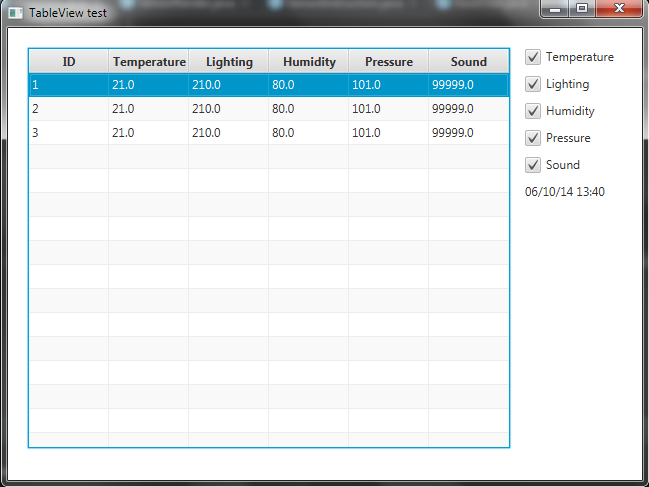
\includegraphics[width=\textwidth]{sprint_1/TableView_Screenshot.png}
\caption{Table View Screenshot}
\end{figure}

The table view is a very simple table of data. In this case we use made-up values to show how it runs and to test its connection to the database. This table view is a clear way to show the exact values and is to be used as an accurate display of sensor values. 

Since we did not receive any hardware (sensors and the central hub) before the sprint was over, we needed to use mock-up values in the database. The table view reads these values and updates itself correctly. These values need to be inputted into the database by hand, since we do not have a client. The last goal, the implementation of the client, was quite difficult without the hardware. It was also made more difficult by the customers request to change the database, resulting in no actual goals achieved in this sprint period.

\subsection{Customer Review}
We have had many meetings with the customer during this sprint. Because the customer is located in Oslo, all of the meetings were held via Skype. On every meeting we showed our progress and explained what we had done so far and what we planned to do next. To do this we used the built in function for sharing screens. 

The customer liked our main idea for the project, but not really the way we wanted to implement it. This led to a lot of changes in our implementation during the sprint. The customer did not want an \gls{SQL} database, but rather to use an online repository and \gls{JSON} files. Furthermore, he did not enjoy the table view, marking it as uninteresting and asking us to remove it. This leaves only one view for the visualization. 

\subsection{Sprint Evaluation}
As stated previously in the results, we have not achieved any goals during this sprint. The customer requested that we should use a different database and this pushed back our work by an entire week. In the end, since we needed to read and learn much about the new technology, we did not manage to implement a fully functioning database and integrate it with the visualizing table. Furthermore, the lack of hardware as well as the database change made it impossible to finish the client on time.

For the future, we will most likely prepare more by listening to the customer and taking his implementation requests before the sprint starts, instead of starting on implementation in a way that suits us. We will also accept no changes after the requests have been placed; while the customers satisfaction is our aim, we also have a very limited time during this project and this will be voiced on our further customer meetings.

We do not feel this sprint was a total failure, even if we have not achieved any of our goals. In reality, most of the implementation will stay the same and once the database is integrated it will change very little, just enough to accompany the integration. Furthermore we have made great strides in the visualization part, by finishing the table view and starting on a prototype for our final visualization, the map view. While the customer did ask us not to show the table view at all during the final presentation, it is still a necessity to have it. Without it we can not be completely sure if all of the values are correctly acquired and updated from the database. We will remove it for the final presentation, but it will remain in internal use until we are done with our implementation.

We have also learned a lot about the architecture and the online database repository (in this specific case, \gls{Cloudant}). We will continue our work in the second sprint to integrate this database correctly into our system.


\end{document}